\documentclass[handout,compress]{beamer}

\usetheme[block=fill]{metropolis}

\usepackage{graphicx} % Allows including images
\usepackage{amsmath,amsfonts,amsthm,amssymb}
\usepackage{color}
\usepackage{xcolor,cancel}
\usepackage{enumitem}
\setitemize{label=\usebeamerfont*{itemize item}%
	\usebeamercolor[fg]{itemize item}
	\usebeamertemplate{itemize item}}
\definecolor{mDarkBrown}{HTML}{604c38}
\definecolor{mDarkTeal}{HTML}{23373b}
\definecolor{mLightBrown}{HTML}{EB811B}
\definecolor{mMediumBrown}{HTML}{C87A2F}
\definecolor{mygreen}{HTML}{98C2B9}
\definecolor{myyellow}{HTML}{DFD79C}
\definecolor{myblue}{HTML}{8CA7CC}
\definecolor{kern}{HTML}{8CC2B7}


\usepackage{float}
\usepackage{framed}
\usepackage{epsfig}
\usepackage{graphicx}
\usepackage{subcaption}
\usepackage{ulem}
\usepackage{hhline}
\usepackage{multirow}
\usepackage{comment}   
\usepackage{bbm}
\usepackage{tikz}   
\def\Put(#1,#2)#3{\leavevmode\makebox(0,0){\put(#1,#2){#3}}}
\newcommand*\mystrut[1]{\vrule width0pt height0pt depth#1\relax}
\newcommand{\eqdef}{\mathbin{\stackrel{\rm def}{=}}}


\newcommand{\bs}[1]{\boldsymbol{#1}}
\newcommand{\bv}[1]{\mathbf{#1}}
\newcommand{\R}{\mathbb{R}}
\newcommand{\E}{\mathbb{E}}

\DeclareMathOperator*{\argmin}{arg\,min}
\DeclareMathOperator*{\argmax}{arg\,max}
\DeclareMathOperator{\nnz}{nnz}
\DeclareMathOperator{\Var}{Var}
\DeclareMathOperator{\sinc}{sinc}
\DeclareMathOperator{\mv}{mv}
\DeclareMathOperator{\sgn}{sgn}
\DeclareMathOperator{\step}{step}
\DeclareMathOperator{\gap}{gap}
\DeclareMathOperator{\poly}{poly}
\DeclareMathOperator{\tr}{tr}
\DeclareMathOperator{\orth}{orth}
\newcommand{\norm}[1]{\|#1\|}
\captionsetup[subfigure]{labelformat=empty}
\captionsetup[figure]{labelformat=empty}
\DeclareMathOperator*{\lmin}{\lambda_{min}}
\DeclareMathOperator*{\lmax}{\lambda_{max}}

\newcommand{\specialcell}[2][c]{%
  \begin{tabular}[#1]{@{}c@{}}#2\end{tabular}}
\newcommand{\specialcellleft}[2][c]{%
\begin{tabular}[#1]{@{}l@{}}#2\end{tabular}
}

\usepackage{tabstackengine}
\stackMath


%----------------------------------------------------------------------------------------
%	TITLE PAGE
%----------------------------------------------------------------------------------------

\title{CS-GY 9223 D: Lecture 2 Supplemental \\ Finish MinHash, Exponential Tail Bounds}
\author{NYU Tandon School of Engineering, Prof. Christopher Musco}
\date{}

\begin{document}

\begin{frame}
	\titlepage 
\end{frame}

\metroset{titleformat=smallcaps}


\begin{frame}
	\frametitle{sketching algorithms}
	\textbf{Abstract architecture of a sketching algorithm:}
	\begin{itemize}
		\item Given a (high dimensional) dataset $D = {d_1, \ldots, d_n}$ with $n$ pieces of data each in $\R^d$.
		\item \textbf{Sketch phase:} For each $i \in 1, \ldots, n$, compute $s_i = C(d_i)$, where $C$ is some compression function and $s_i \in \R^k$ for $k \ll d$.
		\item \textbf{Process phase:} Use (more compact) dataset $s_1, \ldots, s_n$ to approximately compute something about $D$.
	\end{itemize}
	
	\vspace{1em}
	\uncover<4->{
		\begin{columns}
			\begin{column}{.5\textwidth}
				\hspace{1em}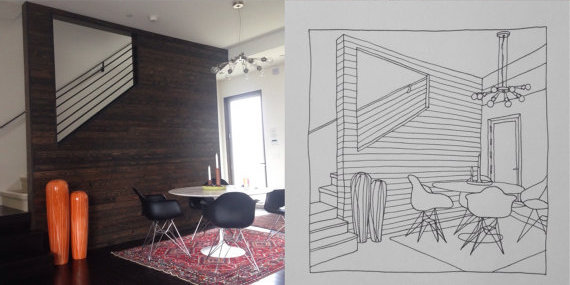
\includegraphics[width=.9\textwidth]{sketch.jpg} 
			\end{column}
			\begin{column}{.5\textwidth}
				Sketching phase is easily distributed, parallelized, etc. Better space complexity, communication complexity, runtime, all at once.
			\end{column}
		\end{columns}	
	}
\end{frame}

\begin{frame}
	\frametitle{similarity estimation}
	\begin{center}
		How does \textbf{Shazam} match a song clip against a library of 8 million songs (32 TB of data) in a fraction of a second?
	\end{center}
	\vspace{-1em}
	\uncover<2->{
		\begin{figure}[h]
			\centering
			\begin{subfigure}[t]{0.35\textwidth}
				\centering
				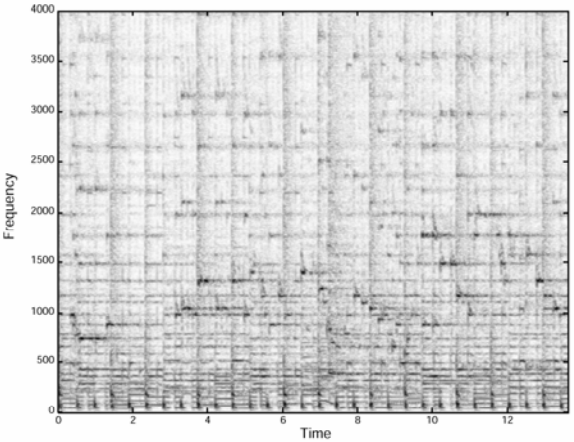
\includegraphics[width=\textwidth]{spectrogram.png}
				\caption{Spectrogram extracted from audio clip.}
			\end{subfigure}
			~
			\begin{subfigure}[t]{0.35\textwidth}
				\centering
				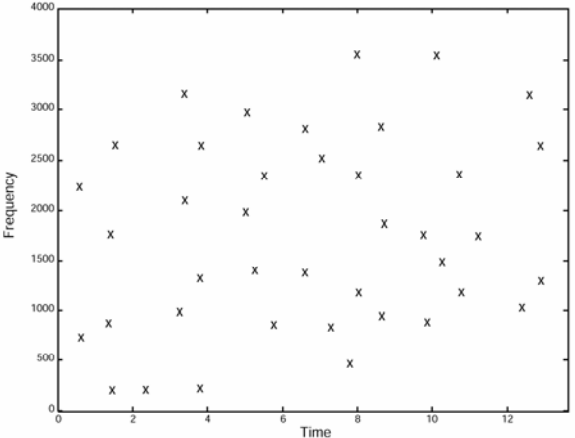
\includegraphics[width=\textwidth]{spectrogramThresh.png}
				\caption{Processed spectrogram: used to construct audio ``fingerprint'' $\textbf{q}\in \{0,1\}^d$.}
			\end{subfigure}
		\end{figure}
		
		\uncover<2->{\vspace{-.5em}
			Each clip is represented by a high dimensional binary vector $\bv{q}$.
			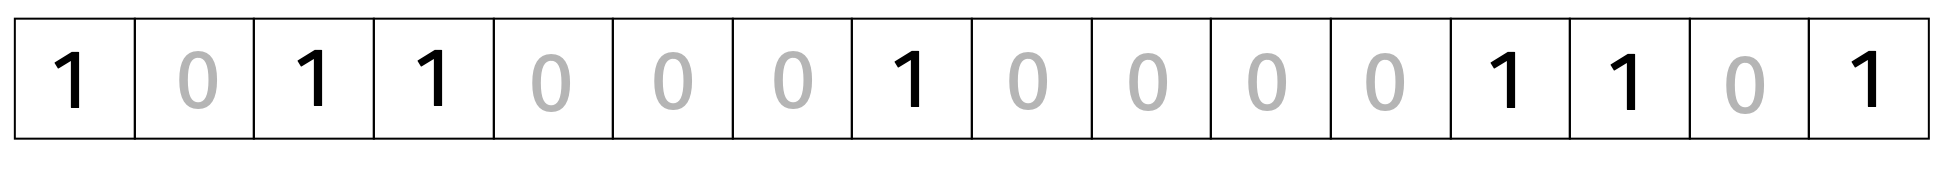
\includegraphics[width=\textwidth]{binaryVector.png}
		}
	}
\end{frame}

\begin{frame}
	\frametitle{similarity estimation}
	\begin{center}
		Given $\textbf{q}$, find any nearby ``fingerprint'' $\bv{y}$  in a database -- i.e. any $\bv{y}$ with $\text{dist}(\bv{y}, \bv{q})$ small. 
	\end{center}
	
	\uncover<2->{
		\textbf{Challenges}:
		\begin{itemize}
			\item Database is possibly huge: $O(nd)$ bits.
			\item Expensive to compute $\text{dist}(\bv{y},\bv{q})$: $O(d)$ time.
		\end{itemize}
	}
\end{frame}

\begin{frame}
	\frametitle{similarity estimation}
	\textbf{Goal:} Design a more compact sketch for comparing $\bv{q}, \bv{y}\in \{0,1\}^d$. Ideally $\ll d$ space/time complexity.
	\uncover<2->{
		\begin{align*}
			C(\textbf{q}) \in \R^k \\	
			C(\textbf{y}) \in \R^k 
		\end{align*}
		\begin{center}
			\vspace{-.5em}
			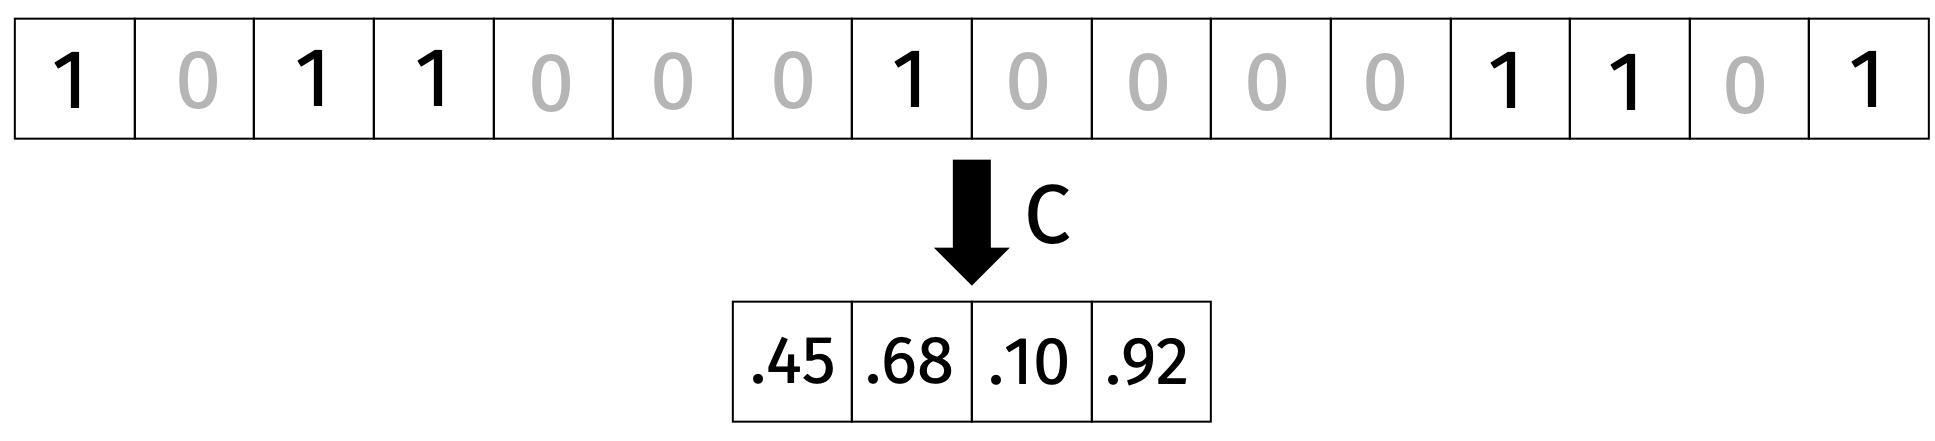
\includegraphics[width=.8\textwidth]{compression.png}
			\vspace{-.5em}
		\end{center}
	}
	\textbf{Homomorphic Compression:}
		
		$C(\bv{q})$ should be similar to $C(\bv{y})$ if $\bv{q}$ is similar to $\bv{y}$.
\end{frame}

\begin{frame}
	\frametitle{jaccard similarity}
	\begin{definition}[Jaccard Similarity]
		\begin{align*}
			J(\bv{q},\bv{y}) = \frac{|\bv{q} \cap \bv{y}|}{|\bv{q} \cup \bv{y}|} = \frac{\text{\# of non-zero entries in common}}{\text{total \# of non-zero entries}}
		\end{align*}
		Natural similarity measure for binary vectors. $0\leq J(\bv{q},\bv{y})\leq 1$.
	\end{definition}

	Can be applied to any data which has a natural binary representation (more than you might think). 
\end{frame}

\begin{frame}
	\frametitle{jaccard similarity for document comparison}
	\textbf{``Bag-of-words'' model:}
	\begin{center}
		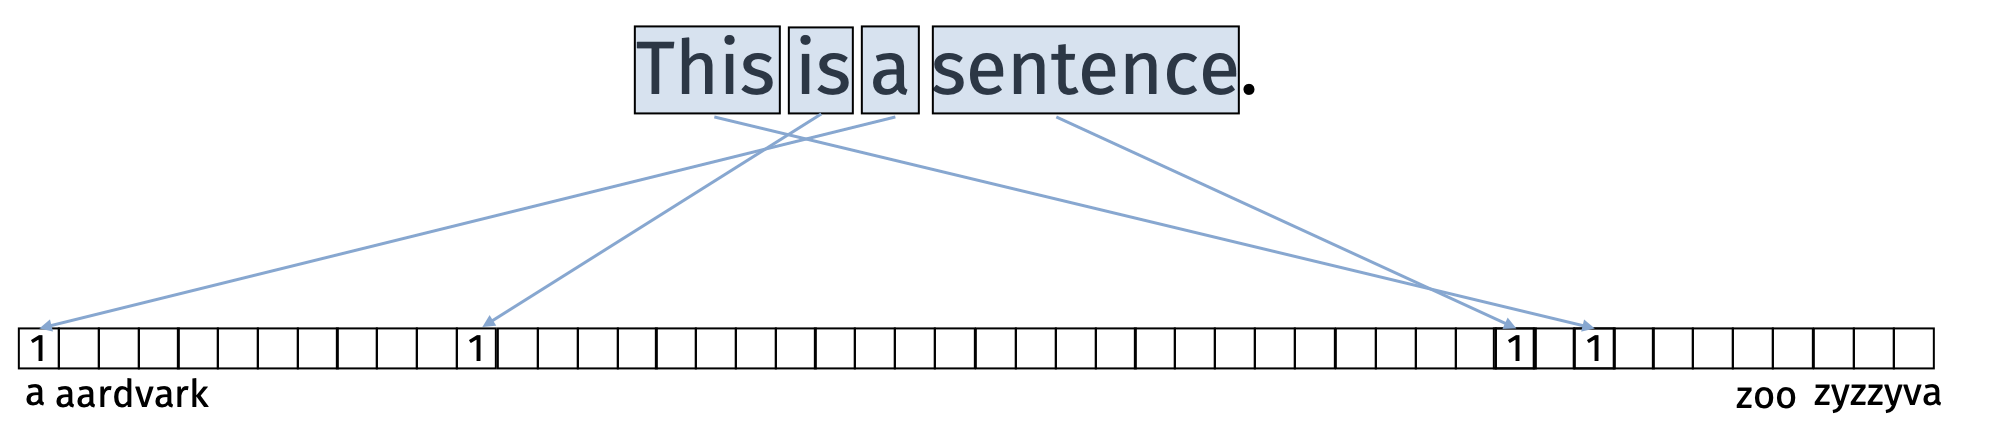
\includegraphics[width=.95\textwidth]{bagofwords.png}
	\end{center}
	
	How many words do a pair of documents have in common?
\end{frame}

\begin{frame}
	\frametitle{jaccard similarity for document comparison}
	\textbf{``Bag-of-words'' model:}
	\begin{center}
		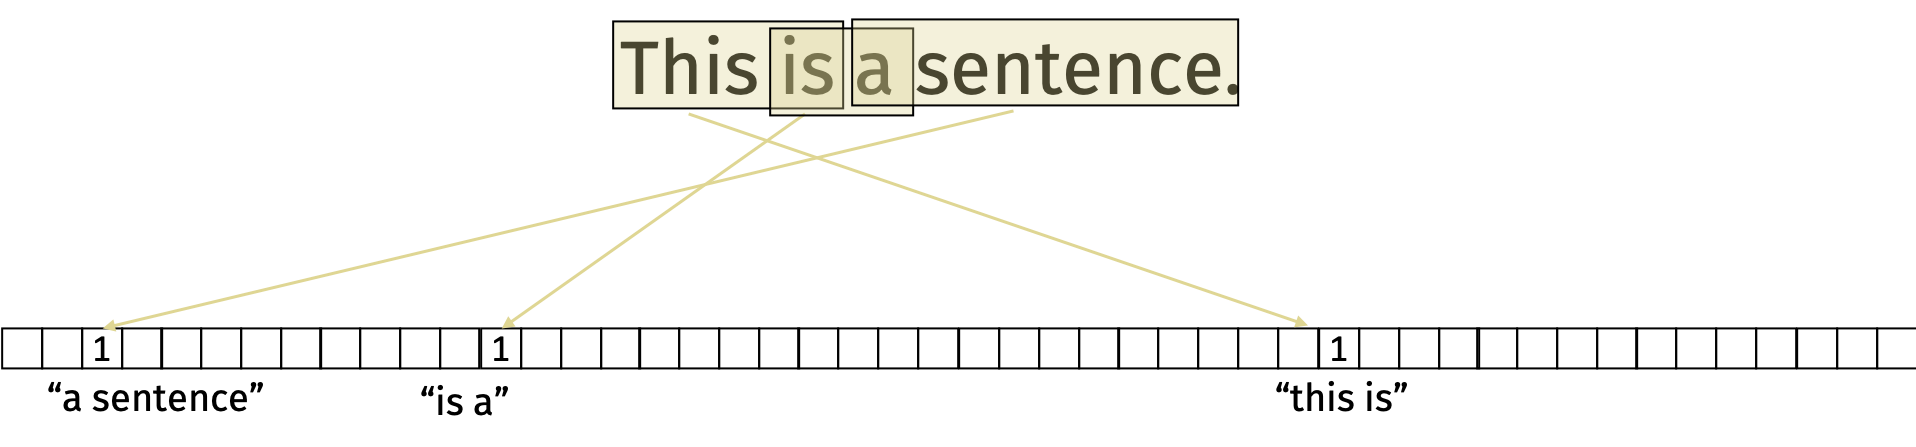
\includegraphics[width=.95\textwidth]{bigrams.png}
	\end{center}
	
	How many bigrams do a pair of documents have in common?
\end{frame}

%\begin{frame}
%	\frametitle{jaccard similarity for seismic data}
%	\begin{center}
%		\vspace{-.5em}
%		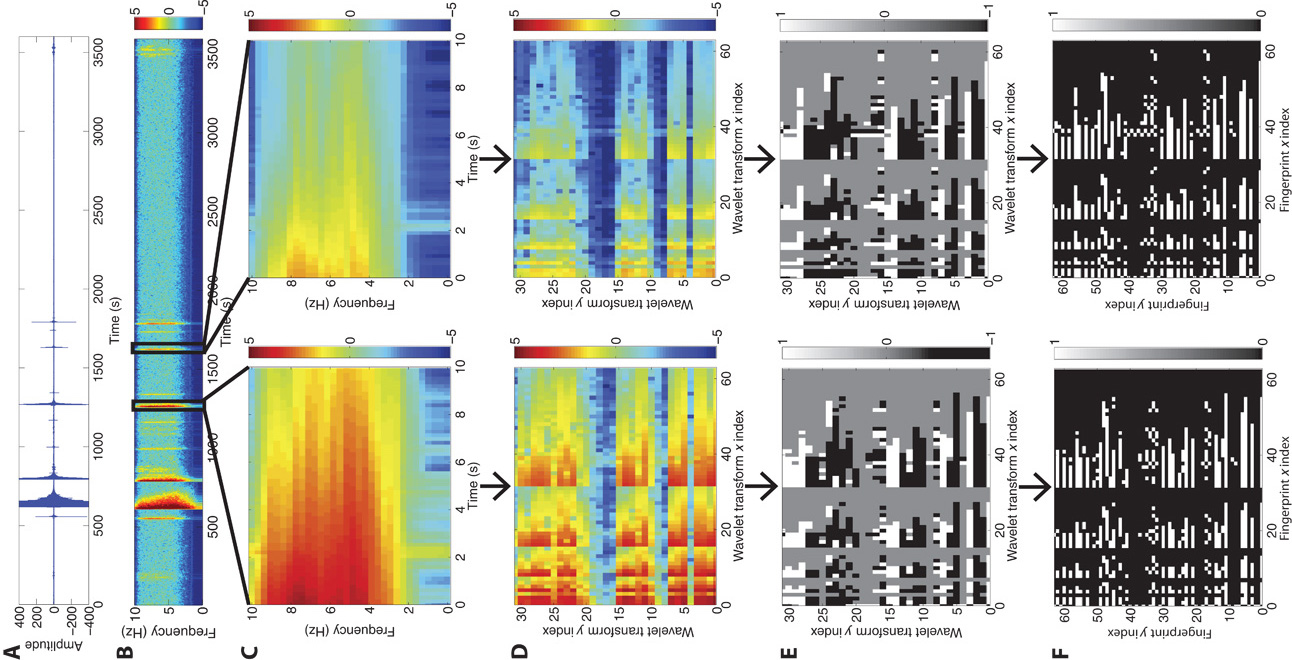
\includegraphics[width=.6\textwidth]{earthquakeFeatures.jpg}
%		
%		\vspace{-.5em}
%		Feature extract pipeline for earthquake data.
%		
%		(see paper by Rong et al. posted on course website)
%	\end{center}
%\end{frame}

\begin{frame}
	\frametitle{applications: document similarity}
	\begin{itemize}
		\item Finding duplicate or new duplicate documents or webpages.
		\item Change detection for high-speed web caches.
		\item Finding near-duplicate emails or customer reviews which could indicate spam.
	\end{itemize}

\begin{center}
	\textbf{Other types of data with a natural binary representation?}
\end{center}
\end{frame}

%	\textbf{Other applications:}
%\begin{itemize}
%	\item Change detection in documents (high speed web caches).
%	\item Analyzing seismic data (matching signatures of earthquakes).
%	\item User recommendations on social networking sites.
%\end{itemize}

\begin{frame}
	\frametitle{similarity estimation}
	\textbf{Goal:} Design a compact sketch $C: \{0,1\}\rightarrow \R^k$:
	\begin{center}
		\vspace{-.5em}
		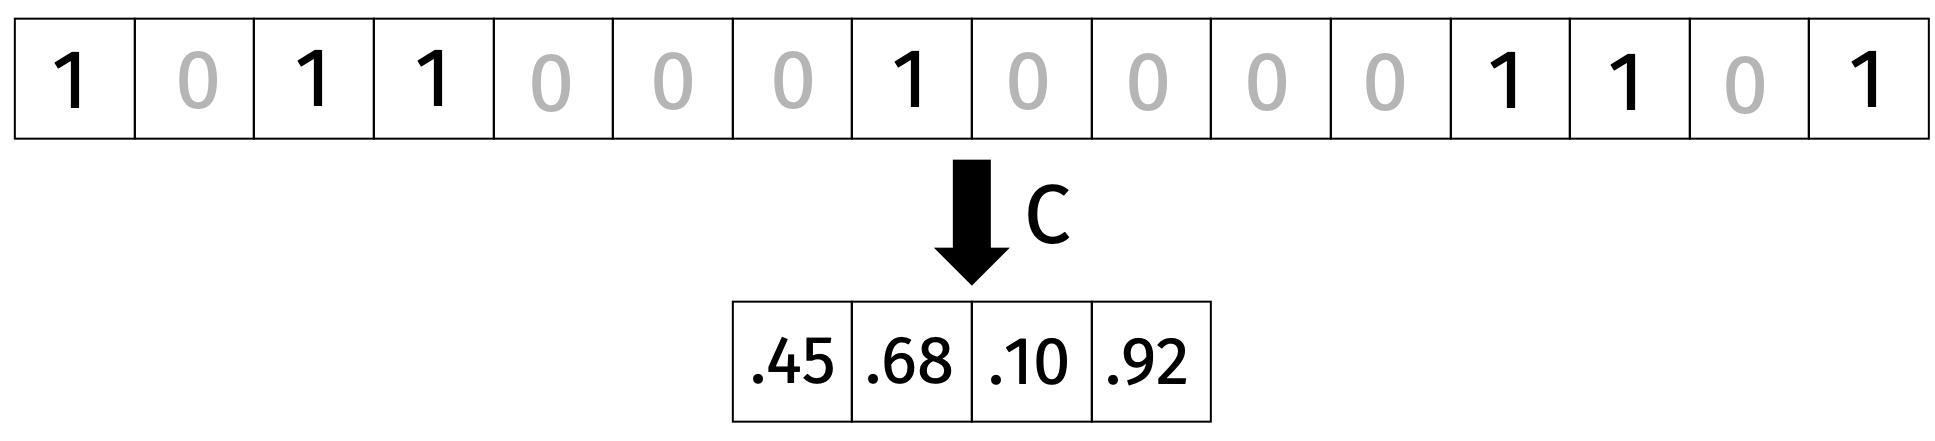
\includegraphics[width=.8\textwidth]{compression.png}
		\vspace{-.5em}
	\end{center}
	\textbf{Homomorphic Compression:} 
	Want to use $C(\bv{q}), C(\bv{y})$ to approximately compute the Jaccard similarity $J(\bv{q},\bv{y})$.
\end{frame}

\begin{frame}
	\frametitle{minhash}
	\textbf{MinHash (Broder, '97)}:
	\begin{itemize}
		\item Choose $k$ random hash functions $h_1, \ldots, h_k: \{1,\ldots, n\} \rightarrow [0,1]$. 
		\item For $i\in 1, \ldots,k$, let $c_i = \min_{j, \bv{q}_j = 1} h_i(j)$.
		\item $C(\bv{q}) = [c_1, \ldots, c_k]$.
	\end{itemize}
	\uncover<2->{\begin{center}
			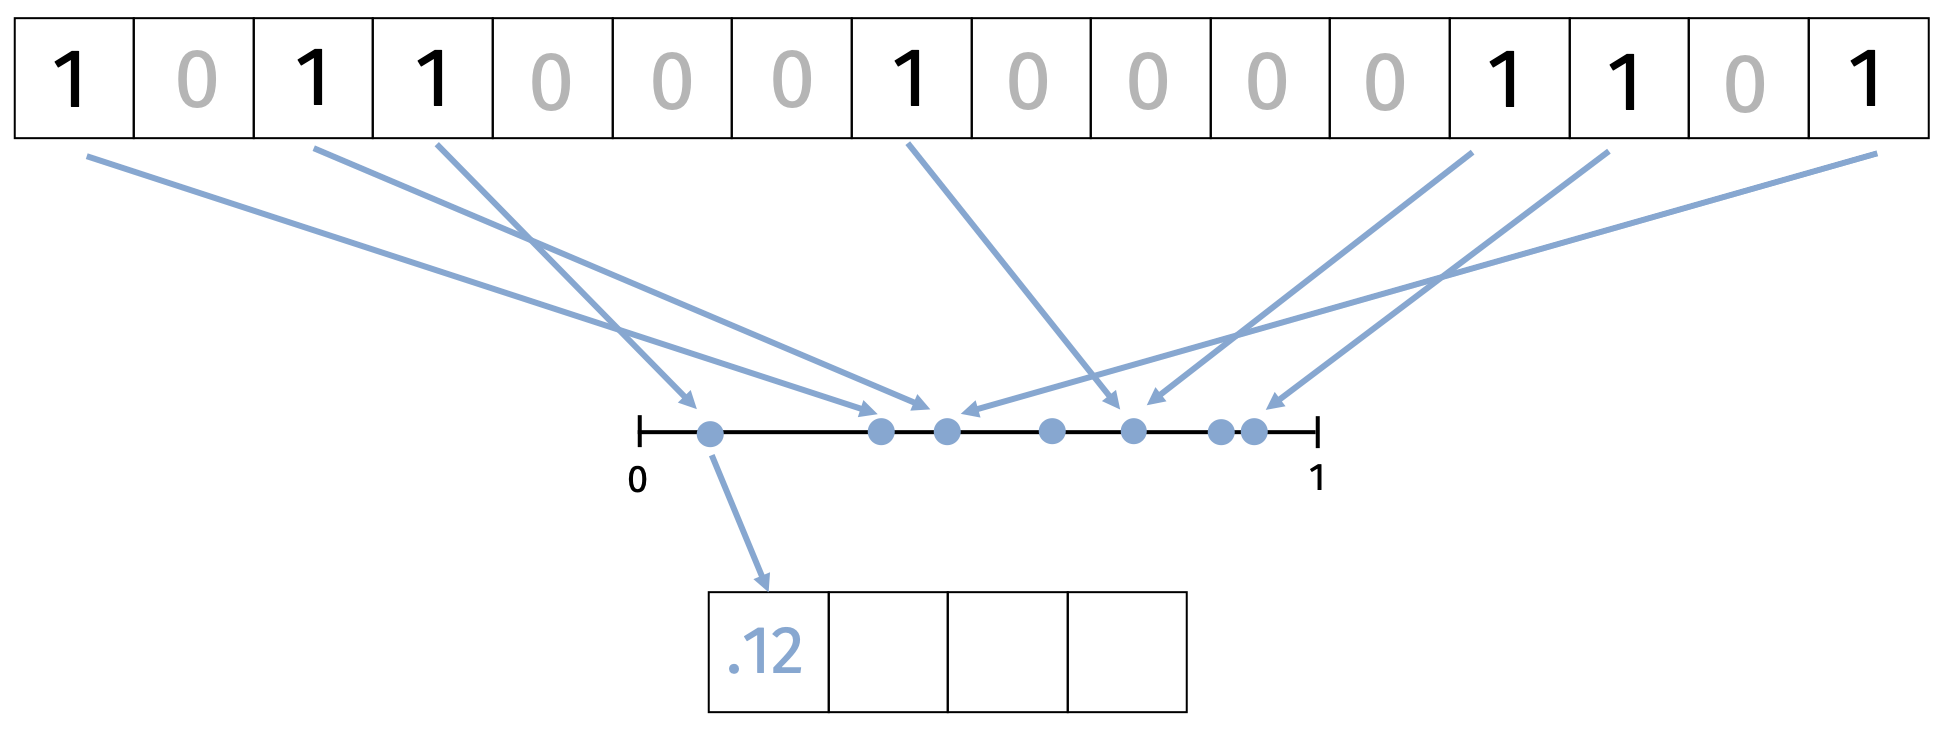
\includegraphics[width=\textwidth]{minHash1.png}	
	\end{center}}
\end{frame}

\begin{frame}
	\frametitle{minhash}
	\begin{itemize}
		\item Choose $k$ random hash functions $h_1, \ldots, h_k: \{1,\ldots, n\} \rightarrow [0,1]$. 
		\item For $i\in 1, \ldots,k$, let $c_i = \min_{j, \bv{q}_j = 1} h_i(j)$.
		\item $C(\bv{q}) = [c_1, \ldots, c_k]$.
	\end{itemize}
	\begin{center}
		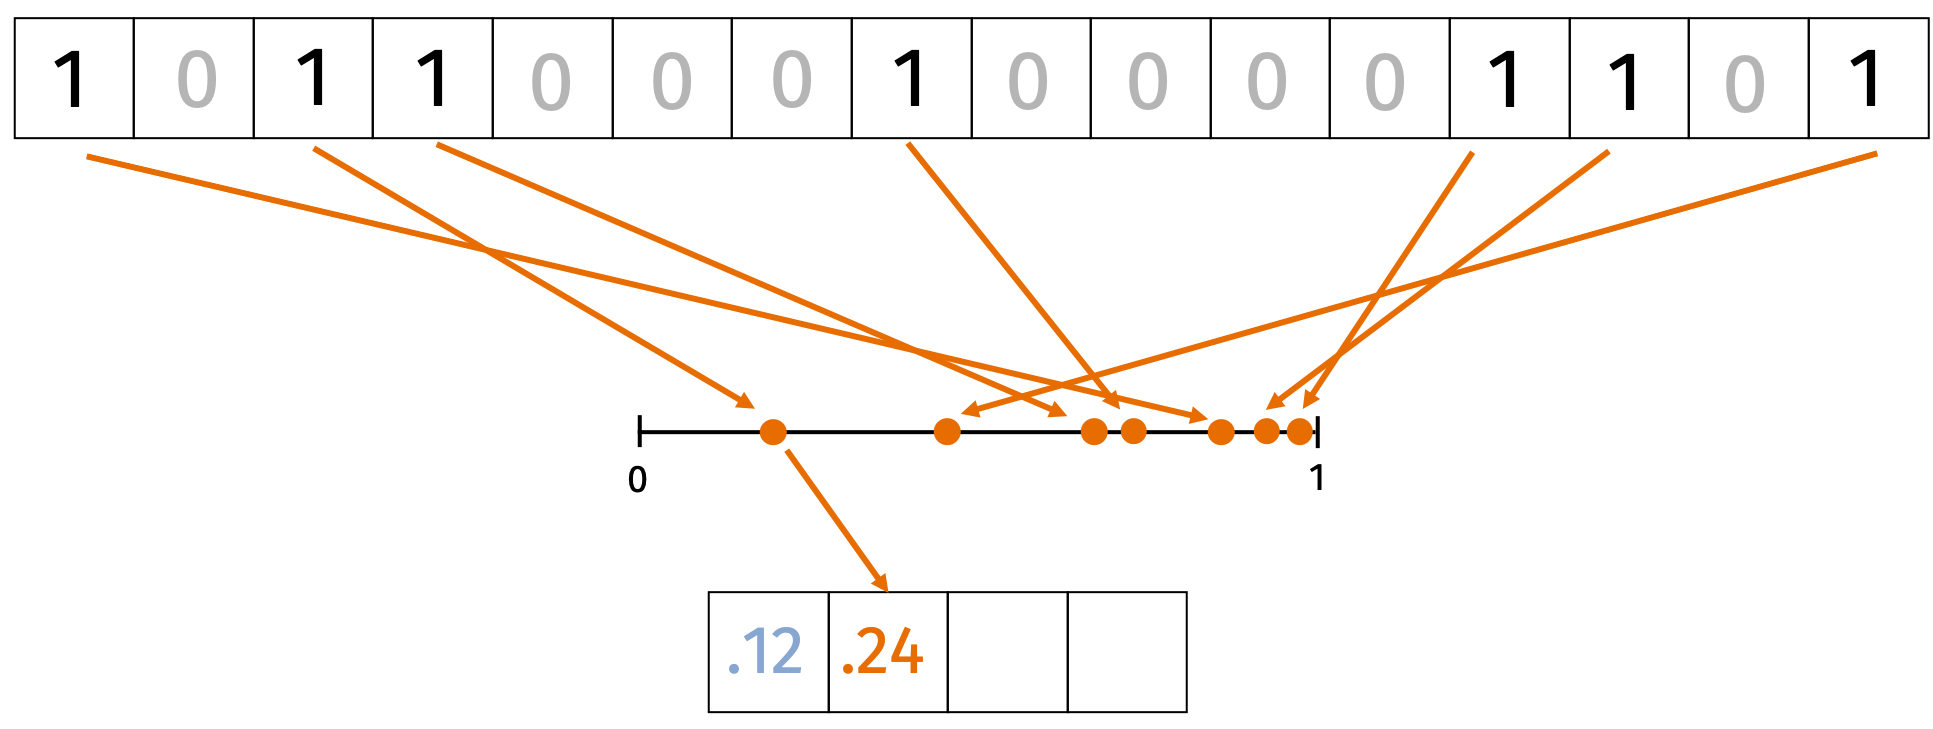
\includegraphics[width=\textwidth]{minHash2.png}	
	\end{center}
\end{frame}

\begin{frame}[t]
	\frametitle{minhash analysis}
	\textbf{Claim:} $\Pr[c_i(\bv{q}) = c_i(\bv{y})] = J(\bv{q},\bv{y})$.	
		\begin{center}
			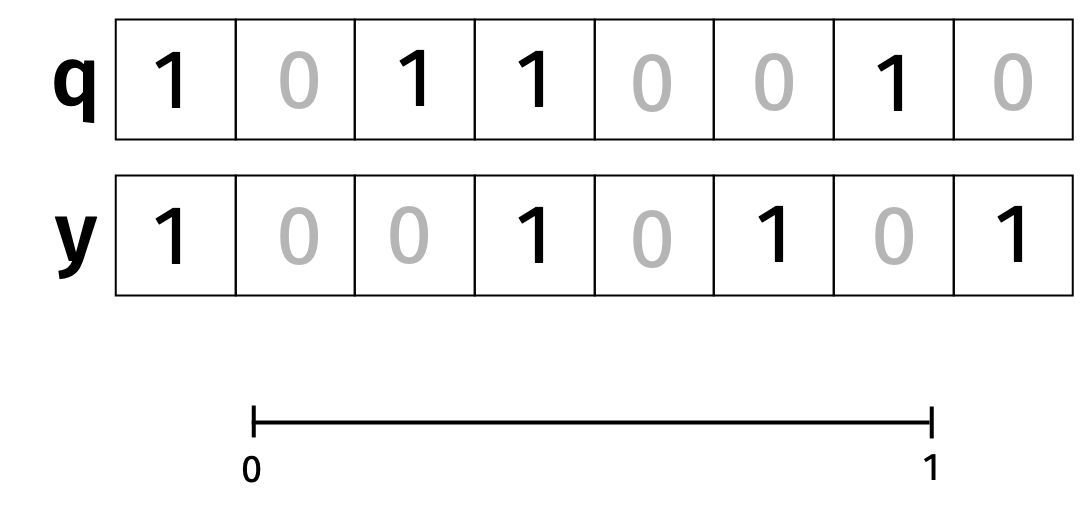
\includegraphics[width=.8\textwidth]{minHashSimple.png}
		\end{center}
\end{frame}

\begin{frame}[t]
	\frametitle{minhash analysis}
	\textbf{Claim:} $\Pr[c_i(\bv{q}) = c_i(\bv{y})] = J(\bv{q},\bv{y})$.	
		\begin{center}
			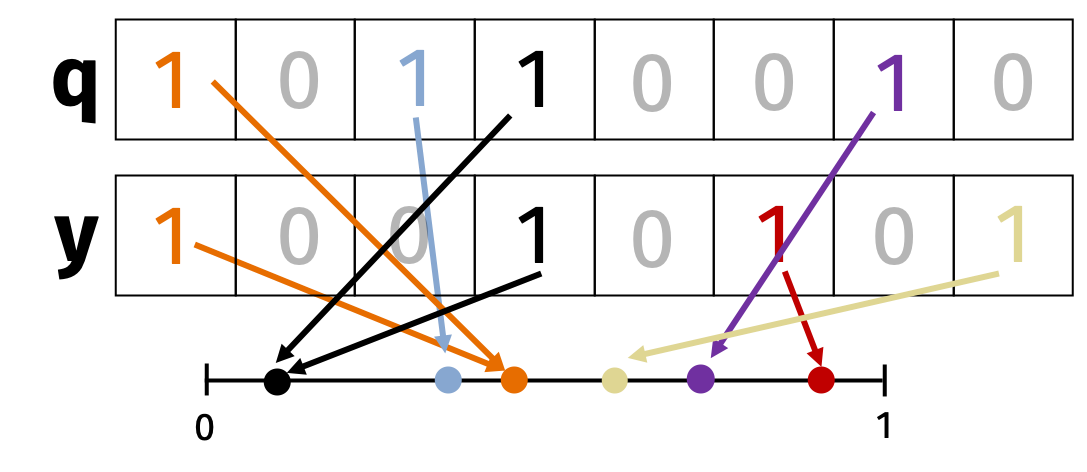
\includegraphics[width=.8\textwidth]{minhash_colored.png}
		\end{center}
	Every non-zero index in $\bv{q}\cup \bv{y}$ is equally likely to produce the lowest hash value.
	$c_i(\bv{q}) = c_i(\bv{y})$ only if this index is 1 in \emph{both} $\bv{q}$ and $\bv{y}$. There are $\bv{q}\cap \bv{y}$ such indices. So:
	\begin{align*}
		\Pr[c_i(\bv{q}) =c_i(\bv{y})]= \frac{\bv{q}\cap \bv{y}}{\bv{q}\cup \bv{y}}  = J(\bv{q},\bv{y})
	\end{align*}
\end{frame}

\begin{frame}
	\frametitle{minhash analysis}
	\textbf{Return:} $\tilde{J} = \frac{1}{k} \sum_{i=1}^k \mathbbm{1}[c_i(\bv{q}) = c_i(\bv{y})]$. 
	
	\textbf{Unbiased estimate for Jaccard similarity:}
	\begin{align*}
		\E \tilde{J} = \hspace{14em}
	\end{align*}

	\begin{center}
		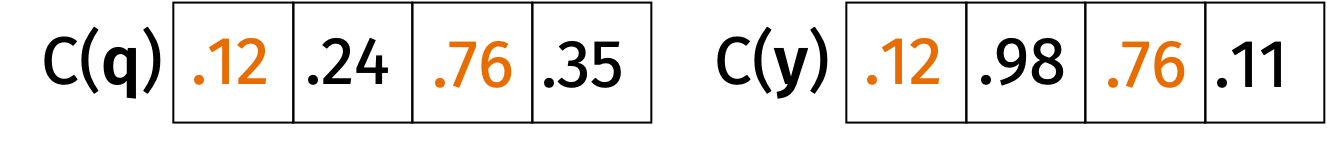
\includegraphics[width=.6\textwidth]{minHashCompare.png}
	\end{center}
The more repetitions, the lower the variance. 
\end{frame}

\begin{frame}
	\frametitle{minhash analysis}
	Let $J = J(\bv{q},\bv{y})$ denote the true Jaccard similarity.
	
	\textbf{Estimator:} $\tilde{J} = \frac{1}{k} \sum_{i=1}^k \mathbbm{1}[c_i(\bv{q}) = c_i(\bv{y})]$. 
	\begin{align*}
		\Var [\tilde{J}] =\hspace{16em}
	\end{align*}
	
	Plug into Chebyshev inequality. How large does $k$ need to be so that with probability $> 1 - \delta$:
	\begin{align*}
		|J-\tilde{J}| \leq \epsilon?
	\end{align*}
\end{frame}

\begin{frame}
	\frametitle{minhash analysis}
	\textbf{Chebyshev inequality:} As long as $\alert{{k = O\left(\frac{1}{\epsilon^2\delta}\right)}}$, then with prob. $1-\delta$,
	\begin{align*}
		J(\bv{q}, \bv{y}) -\epsilon \leq \tilde{J}\left(C(\bv{q}),C(\bv{y})\right)   \leq J(\bv{q}, \bv{y}) + \epsilon. 
	\end{align*}
		\begin{center}
			And $\tilde{J}$ only takes $O(k)$ time to compute! \alert{\textbf{Independent}} of original fingerprint dimension $d$.
		\end{center}	
	
	However, a linear dependence on $\frac{1}{\delta}$ is not good! Suppose we have a database of $n$ songs slips, and Shazam wants to ensure the similarity between a query $\bv{q}$ and \emph{every song clip} $\bv{y}$ is approximated well. 
	
	We would need $\delta \approx 1/n$. I.e. our compression need to use $k = O(n/\epsilon^2)$ dimensions, which is far too large!
\end{frame}

\begin{frame}
	\frametitle{beyond chebyshev}
	\textbf{Motivating question:} Is Chebyshev's Inequality tight?
	\vspace{-.5em}
		\begin{figure}
			\centering
			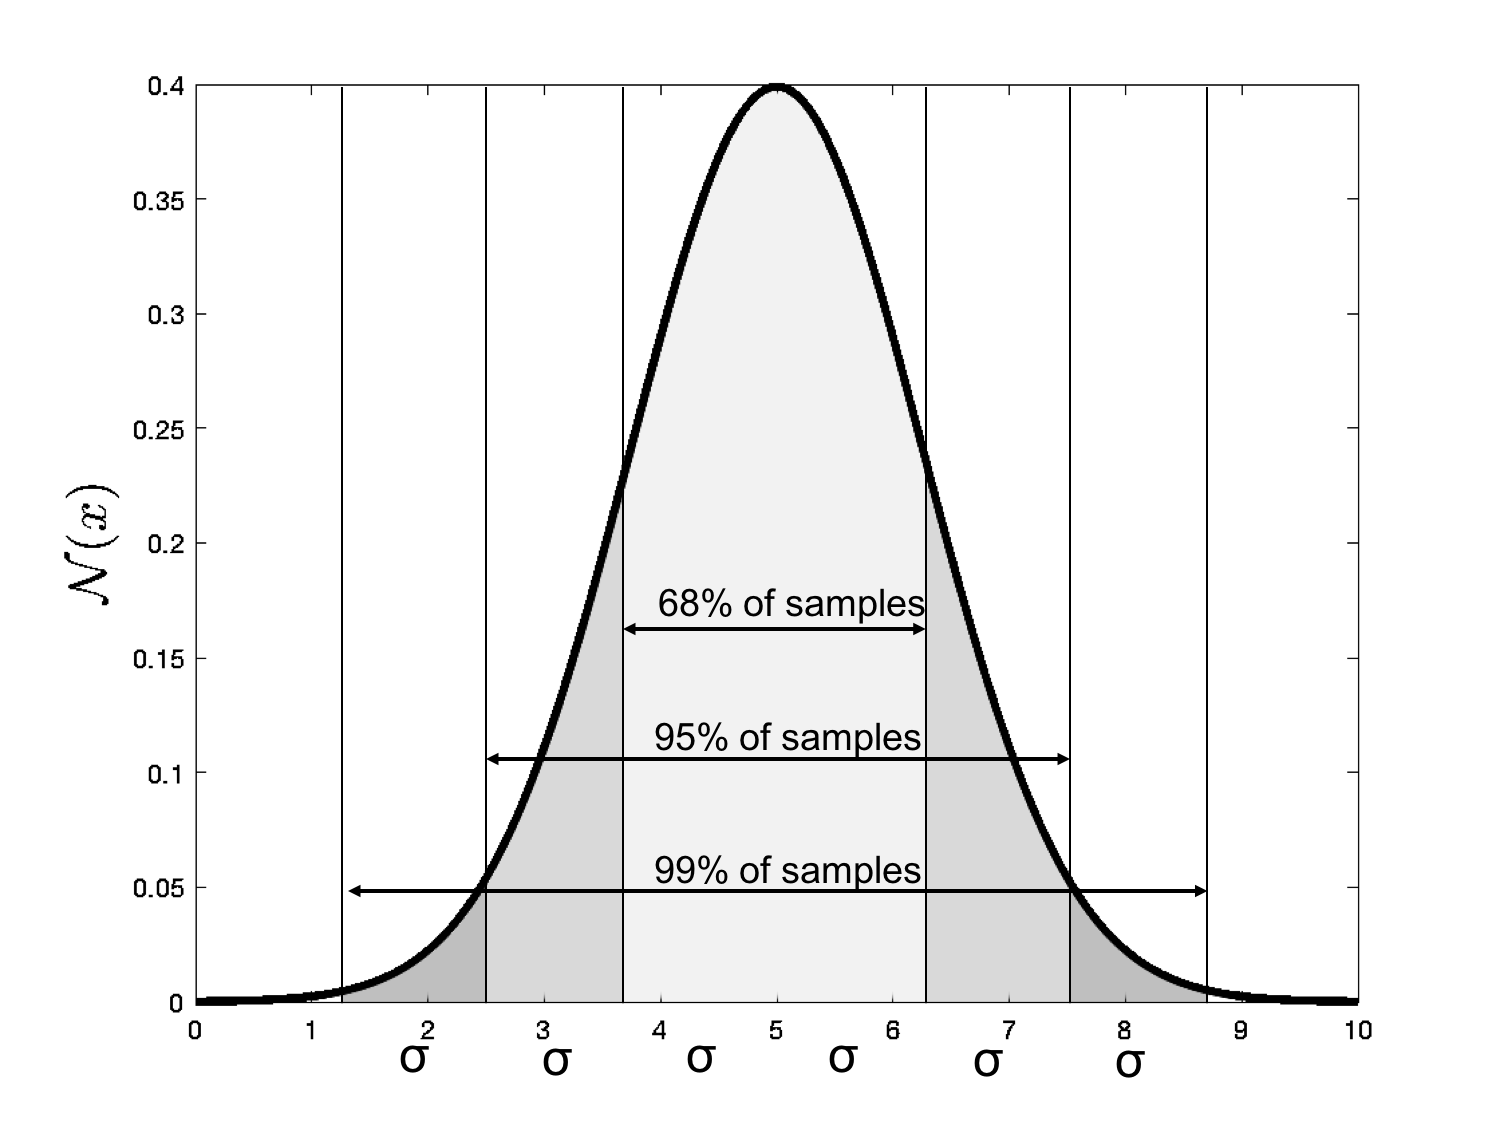
\includegraphics[width=0.4\textwidth]{689599rule.png}
			\caption{68-95-99 rule for Gaussian bell-curve. \alert{$\mathbf{X\sim N(0,\sigma^2)}$}}
		\end{figure}
	
		\begin{columns}
			\begin{column}{.5\textwidth}
				\small
				\textbf{Chebyshev's Inequality:}
				\vspace{-.5em}
				\begin{align*}
					\Pr\left(|X - \E[X]| \geq 1\sigma \right) &\leq 100\% \\
					\Pr\left(|X - \E[X]| \geq 2\sigma \right) &\leq 25\% \\
					\Pr\left(|X - \E[X]| \geq 3\sigma \right) &\leq 11\% \\
					\Pr\left(|X - \E[X]| \geq 4\sigma \right) &\leq 6\%.
				\end{align*}
			\end{column}
			\begin{column}{.5\textwidth}
				\small
				\textbf{Truth:}
				\vspace{-.5em}
				\begin{align*}
					\Pr\left(|X - \E[X]| \geq 1\sigma \right) &\approx 32\% \\
					\Pr\left(|X - \E[X]| \geq 2\sigma \right) &\approx 5\% \\
					\Pr\left(|X - \E[X]| \geq 3\sigma \right) &\approx 1\% \\
					\Pr\left(|X - \E[X]| \geq 4\sigma \right) &\approx .01\%
				\end{align*}
			\end{column}
		\end{columns}
\end{frame}

\begin{frame}
	\frametitle{gaussian concentration}
	For $X \sim \mathcal{N}(\mu,\sigma^2)$:
	\begin{align*}
		\Pr[X = \mu \pm x] = \frac{1}{\sigma\sqrt{2\pi}} \alert{\mathbf{e^{-x^2/2\sigma^2}}}
	\end{align*}
		\vspace{-1em}
		\begin{lemma}[Guassian Tail Bound]
			For $X \sim \mathcal{N}(\mu,\sigma^2)$:
			\begin{align*}
				\Pr[|X - \E X| \geq \alpha\cdot\sigma] \leq O(e^{-\alpha^2/2}).
			\end{align*}
		\end{lemma}
		\begin{figure}
			\begin{subfigure}[t]{0.3\textwidth}
				\centering
				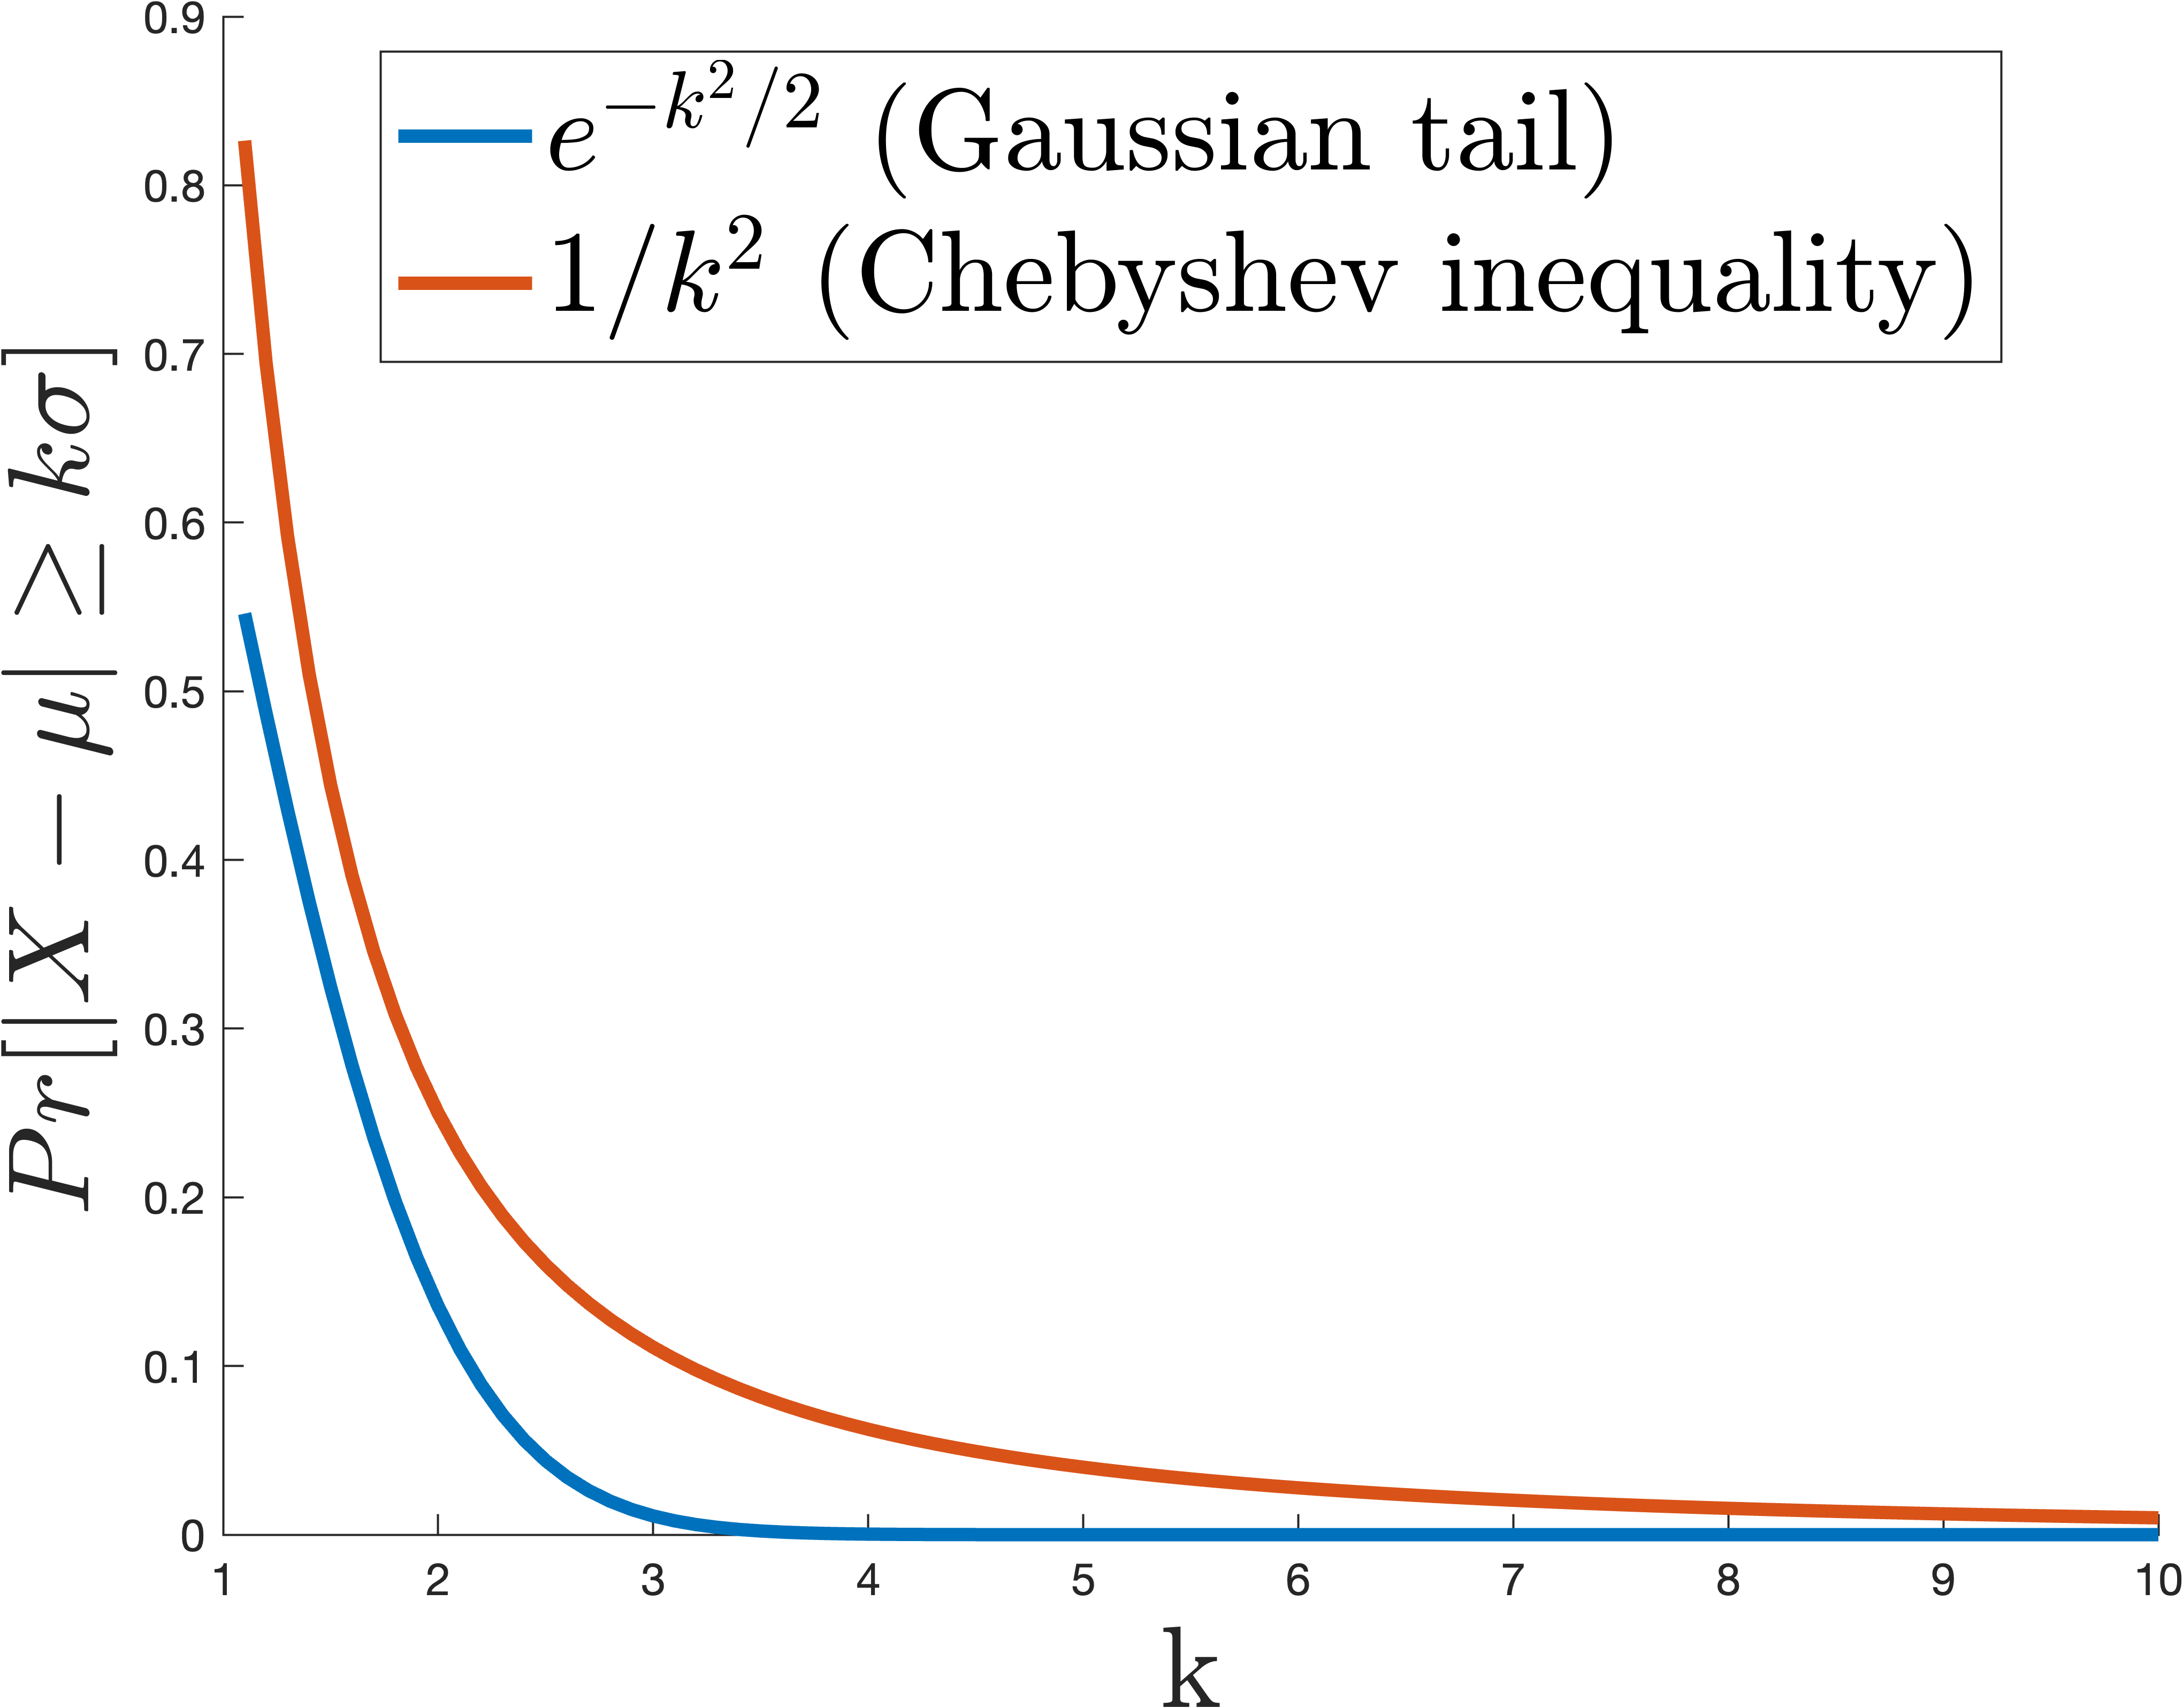
\includegraphics[width=\textwidth]{standardScale.png}
				\caption{Standard $y$-scale.}
			\end{subfigure}
			\hspace{3em}
			\begin{subfigure}[t]{0.3\textwidth}
				\centering
				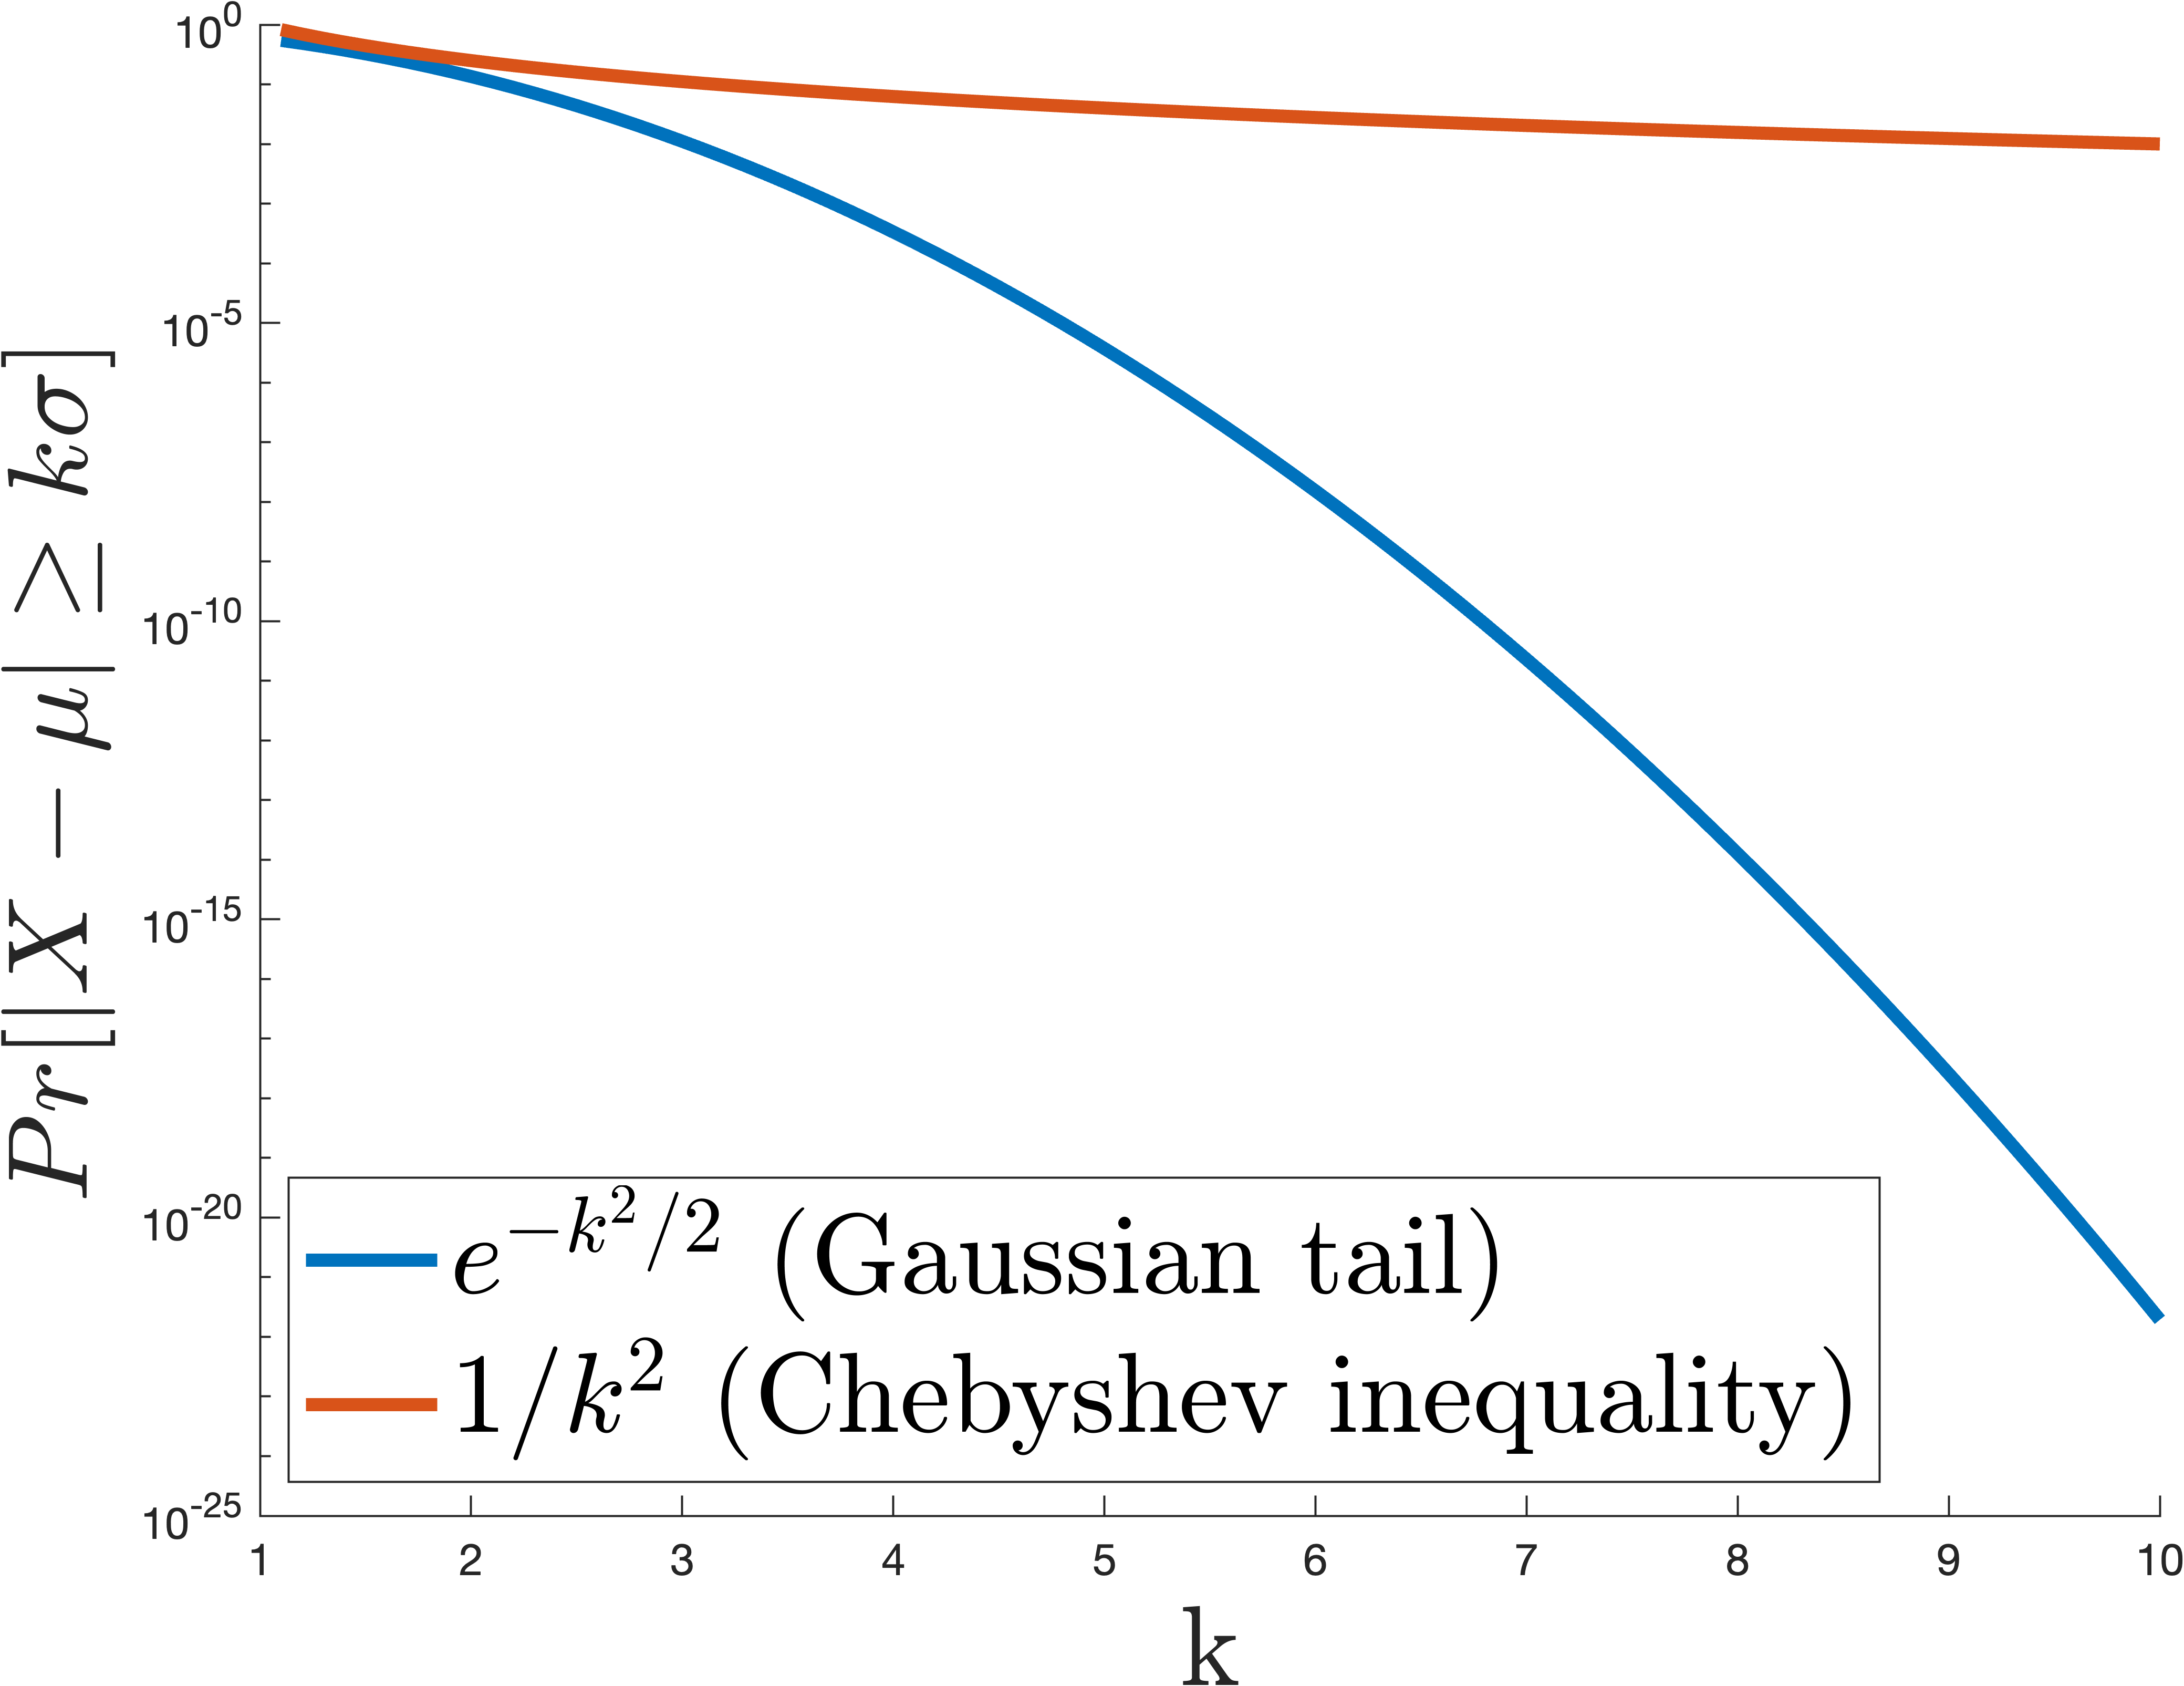
\includegraphics[width=\textwidth]{logScale.png}
				\caption{Logarithmic $y$-scale.}
			\end{subfigure}
		\end{figure}
	
\end{frame}

\begin{frame}
	\frametitle{gaussian concentration}
	\textbf{Takeaway:} Gaussian random variables concentrate much tighter around their expectation than variance alone  predicts.
	
		\begin{center}
			\alert{Why does this matter for algorithm design?}
		\end{center}
\end{frame}

\begin{frame}
	\frametitle{central limit theorem}
	\begin{theorem}[CLT -- Informal]
		Any sum of \alert{independent}, \alert{(identically distributed)}  r.v.'s $X_1,  \ldots, X_k$ with mean $\mu$ and finite variance $\sigma^2$ converges to a Gaussian r.v. with mean $k\cdot\mu$ and variance $k\cdot\sigma^2$, as $k\rightarrow \infty$.
		\vspace{-.5em}
		\begin{align*}
			S = \sum_{i=1}^n X_i \Longrightarrow \mathcal{N}(k\cdot\mu, k\cdot\sigma^2).
		\end{align*}	
		\vspace{-.5em}	
	\end{theorem}
	\vspace{-.5em}	
		\begin{figure}
			\begin{subfigure}[t]{0.4\textwidth}
				\centering
				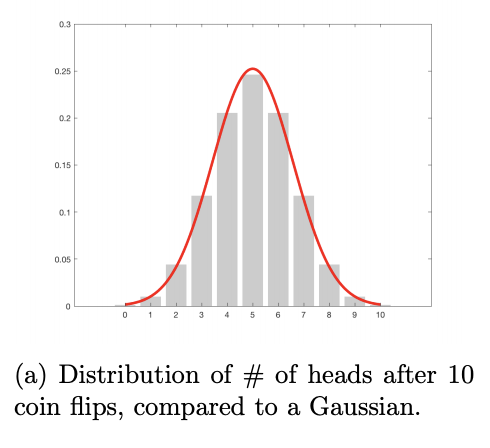
\includegraphics[width=\textwidth]{cltWide.png}
			\end{subfigure}
			\hspace{4em}
			\begin{subfigure}[t]{0.4\textwidth}
				\centering
				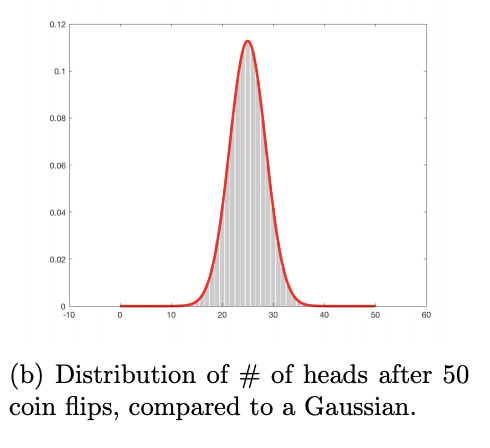
\includegraphics[width=\textwidth]{cltSkinny.png}
			\end{subfigure}
		\end{figure}
\end{frame}

\begin{frame}
	\frametitle{independence}
	\begin{definition}[Mutual Independence]
		Random variables $X_1, \ldots, X_k$ are \emph{mutually independent} if, for all possible values $v_1, \ldots, v_k$,
		\begin{align*}
			\Pr[X_1 = v_1, \ldots, X_k = v_k] = 	\Pr[X_1 = v_1]\cdot\ldots \cdot\Pr[X_k = v_k]
		\end{align*}
	\end{definition}
	\begin{center}
		\uncover<2->{\textbf{Strictly stronger than pairwise independence.}}
	\end{center}
\end{frame}

\begin{frame}
	\frametitle{exercise}
	\small 
	You have access to a coin and want to determine if it's $\epsilon$-close to unbiased. To do so, you flip the coin repeatedly and check that the ratio of heads flips is between $1/2 - \epsilon$ and $1/2 + \epsilon$. If it is not, you reject the coin as overly biased. 
	
	\begin{enumerate}[label=(\alph*)]
		\item How many flips $k$ are required so that, with probability $(1-\delta)$, you do not accidentally reject a truly unbiased coin? The solution with depend on $\epsilon$ and $\delta$.
	\end{enumerate}
	
	%	As in the previous lecture, we we would like to use concentration bounds to study the randomized load balancing problem. $n$ jobs are distributed randomly to $n$ servers using a hash function. Let $S_i$ be the number of jobs sent to server $i$. 
	%	\begin{enumerate}[label=(\alph*)]
	%		\item Using the CLT and our lemma for Gaussian concentration, estimate a bound for $\max_i[S_i]$. For example, your bound should take the form: $\Pr[max_i S_i \geq \alert{\textbf{B}}] \leq 1/10$. What's the smallest value of $\textbf{\alert{B}}$ you should hope to achieve? 
	%		\item Last class we proved the above bound with $\textbf{B} = O(\sqrt{n})$ using Chebyshev inequality. How does your bound compare?
	%	\end{enumerate}
	
	For this problem, we will assume the CLT holds exactly for a sum of independent random variables -- i.e., that this sum looks exactly like a Gaussian random variable.
	\begin{lemma}[Guassian Tail Bound]
		For $X \sim \mathcal{N}(\mu,\sigma^2)$:
		\begin{align*}
			\Pr[|X - \E X| \geq \alpha\cdot \sigma] \leq O(e^{-\alpha^2/2}).
		\end{align*}
	\end{lemma}
\end{frame}

\begin{frame}
	\frametitle{back-of-the-envelop calculation}
	
\includegraphics[width=.9\textwidth]{envelope.jpg}
\end{frame}


\begin{frame}
	\frametitle{quantitative versions of the clt}
	\textbf{These back-of-the-envelop calculations can be made rigorous!}
	\uncover<2->{\textbf{\alert{Lots of different ``versions'' of bound which do so.}}
		\begin{center}
			\begin{itemize}
				\item Chernoff bound
				\item Bernstein bound
				\item Hoeffding bound
				\item $\ldots$
			\end{itemize}
			Different assumptions on random varibles (e.g. binary, bounded, i.i.d), different forms (additive vs. multiplicative error), etc. \textbf{Wikipedia is your friend.}
		\end{center}
	}
\end{frame}

\begin{frame}
	\frametitle{quantitative versions of the clt}
	\begin{theorem}[Chernoff Bound]
		Let $X_1,X_2,\ldots,X_k$ be independent $\{0,1\}$-valued random variables and let
		$p_i = \E[X_i]$, where $0<p_i<1$.
		Then the sum $S = \sum_{i=1}^{k} X_i$, which has mean
		$\mu = \sum_{i=1}^{k} p_i$, satisfies
		\begin{align*}
			\Pr[S \geq (1+\epsilon)\mu] \leq e^{\frac{-\epsilon^2\mu}{2+ \epsilon}}.
		\end{align*}
	and for $0<\epsilon <1$
		\begin{align*}
		\Pr[S \leq (1-\epsilon)\mu] \leq e^{\frac{-\epsilon^2\mu}{2}}.
	\end{align*}
	\end{theorem} 
\end{frame}

\begin{frame}
	\frametitle{quantitative versions of the clt}
	\begin{theorem}[Bernstein Inequality]
		Let $X_1, X_2, \ldots, X_k$ be independent random variables with each $X_i \in [-1,1]$.
		Let $\mu_i =\E[X_i]$ and $\sigma_i^2 = \Var[X_i]$. Let  $\mu =\sum_i \mu_i$ and $\sigma^2 =\sum_i \sigma_i^2$. Then, for $\alpha \leq \frac{1}{2}\sigma$, $S =\sum_i X_i$ satisfies
		$$\Pr[|S - \mu| > \alpha\cdot \sigma] \leq  2 \exp(-\frac{\alpha^2}{4}).$$
	\end{theorem}
\end{frame}

\begin{frame}
	\frametitle{quantitative versions of the clt}
	\begin{theorem}[Hoeffding Inequality]
		Let $X_1, X_2, \ldots, X_k$ be independent random variables with each $X_i \in [a_i,b_i]$.
		Let $\mu_i =\E[X_i]$ and $\mu =\sum_i \mu_i$. Then, for any $\alpha > 0$, $S =\sum_i X_i$ satisfies:
		$$\Pr[|S - \mu| > \alpha] \leq  2 \exp(-\frac{\alpha^2}{\sum_{i=1}^k (b_i-a_i)^2}).$$
	\end{theorem}
\end{frame}

\begin{frame}
	\frametitle{how are these bounds proven?}
	Variance is a natural \emph{measure of central tendency}, but there are others. 
	\begin{align*}
	q^\text{th} \text{ central moment: } \E[(X-\E X)^q]
	\end{align*}
$k = 2$ gives the variance. Proof of Chebyshev's applies Markov's inequality to the random variable $(X - \E X)^2)$.

\textbf{Idea in brief:} Apply Markov's inequality to $\E[(X-\E X)^q$ for larger $q$, or more generally to $f(X-\E X)$ for some other non-negative function $f$. E.g., to $\exp(X-\E X)$. 

We will explore this approach in the next problem set.
	
\end{frame}

\begin{frame}
	\frametitle{chernoff bound application}
	\small
	\textbf{Sample Application:} Flip biased coin $k$ times: i.e. the coin is heads with probability $b$. As long as $k \geq O\left(\frac{\log(1/\delta)}{\epsilon^2}\right)$,
	\vspace{-.5em}
	\begin{align*}
		\Pr[|\text{\# heads} - b\cdot k| \geq \epsilon k] \leq \delta 
	\end{align*}
	
	\textbf{Setup:}
	Let $X_i = \mathbbm{1}[i^\text{th} \text{ flip is heads}]$. Want bound probability that  $\sum_{i=1}^k X_i$ deviates from it's expectation.
	
	\textbf{Corollary of Chernoff bound}: Let $S = \sum_{i=1}^k X_i$ and $\mu = \E[S]$. For $0< \Delta < 1$, 
	\vspace{-.75em}
	\begin{align*}
		\Pr[|S - \mu| \geq \Delta \mu] \leq 2e^{-\Delta^2 \mu/3}
	\end{align*} 
\vspace{6em}
\end{frame}

\begin{frame}
	\frametitle{chernoff bound application}
	\textbf{Sample Application:} Flip biased coin $k$ times: i.e. the coin is heads with probability $b$. As long as $k \geq O\left(\frac{\log(1/\delta)}{\epsilon^2}\right)$,
	\begin{align*}
		\Pr[|\text{\# heads} - b\cdot k| \geq \epsilon k] \leq \delta 
	\end{align*}
	
	
	
	Pay very little for higher probability -- if you increase the number of coin flips by 2x, $\delta$ goes from $1/10 \rightarrow 1/100 \rightarrow 1/10000$
\end{frame}

\begin{frame}
	\frametitle{application to minhash}
	Let $J = J(\bv{q},\bv{y})$ denote the true Jaccard similarity.
	
	\textbf{Estimator:} $\tilde{J} = \frac{1}{k} \sum_{i=1}^k \mathbbm{1}[c_i(\bv{q}) = c_i(\bv{y})]$. 
	
	By the analysis above,
	\begin{align*}
		\Pr[|\tilde{J} - J| \geq \epsilon] = \Pr[|\tilde{J} \cdot k - J\cdot k| \geq \epsilon k] \leq \delta 
	\end{align*} 
	as long as $k = O\left(\frac{\log(1/\delta)}{\epsilon^2}\right)$. 
	
	Much better than the $k = O\left(\frac{1}{\delta\epsilon^2}\right)$.
	
	For example, if we had a data base of $n=1,000,000$ songs, setting $\delta = \frac{1}{n}$ would only require space depending on $\log(n) \approx 14$, instead of on $n=1,000,000$.  
	
\end{frame}


\begin{frame}
	\frametitle{load balancing}
	\small
	As in the first video lecture, we want to use concentration bounds to study the randomized load balancing problem. $n$ jobs are distributed randomly to $n$ servers using a hash function. Let $S_i$ be the number of jobs sent to server $i$.  What's the smallest $\alert{\mathbf{B}}$ for which we can prove:
	\begin{align*}
		\Pr[max_i S_i \geq \alert{\mathbf{B}}] \leq 1/10
	\end{align*}
	\vspace{-1em}
	\begin{center}
		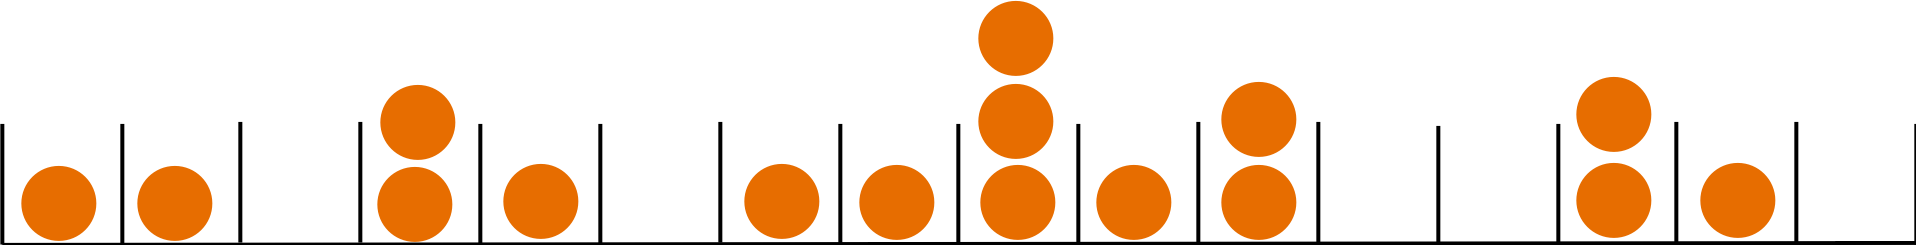
\includegraphics[width=.6\textwidth]{ballsinbins.png}
	\end{center}
	
		\textbf{Recall:} Suffices to prove that, for any $i$, $\Pr[ S_i \geq {\mathbf{B}}] \leq 1/10n$:
		\begin{align*}
			\Pr[max_i S_i \geq {\mathbf{B}}] &= \Pr[S_1 \geq {\mathbf{B}} \text{ or } \ldots \text{ or } S_1 \geq {\mathbf{B}}] \\
			&\leq \Pr[S_1 \geq {\mathbf{B}}] + \ldots + \Pr[S_n \geq {\mathbf{B}}] \text{\hspace{1em} (union bound)}.
		\end{align*}
\end{frame}

\begin{frame}[t]
	\frametitle{load balancing}
	\begin{theorem}[Chernoff Bound]
		Let $X_1,X_2,\ldots,X_n$ be independent $\{0,1\}$-valued random variables and let
		$p_i = \E[X_i]$, where $0<p_i<1$.
		Then the sum $S = \sum_{j=1}^{n} X_i$, which has mean
		$\mu = \sum_{j=1}^{n} p_i$, satisfies
		\begin{align*}
			\Pr[X \geq (1+\epsilon)\mu] \leq e^{\frac{-\epsilon^2\mu}{3 + 3\epsilon}}.
		\end{align*}
	\end{theorem} 
	Consider a single bin. Let $X_j = \mathbbm{1}[\text{ball $j$ lands in that bin}]$. $\E[X_j] = \frac{1}{n}$, so $\mu = 1$. 
	\begin{align*}
		\Pr[S \geq (1+c\log n)\mu] \leq e^{\frac{-c^2\log^2 n}{c + c\log n}} \leq e^{\frac{-c\log^2 n}{2\log n}} \leq e^{-.5c\log n} \leq \frac{1}{10n},
	\end{align*}
	for sufficiently large $c$

\end{frame}

\begin{frame}
	\frametitle{power of two choices}
	\begin{center}\alert{\textbf{So max load for randomized load balancing is $O(\log n)$!}} Best we could prove with Chebyshev's was $O(\sqrt{n})$. \end{center}
	
	\textbf{Power of 2 Choices:} Instead of assigning job to random server, choose 2 random servers and assign to the least loaded. With probability $1/10$ the maximum load is bounded by:
	\begin{enumerate}[label=(\alph*)]
		\item $O(\log n)$
		\item $O(\sqrt{\log n})$
		\item $O(\log log n)$
		\item $O(1)$
	\end{enumerate}
\end{frame}


\end{document} 








